\iffalse
There are a great many natural phenomena which involve the diffusion of small particles through solids; interface problems, such as the growth of a titanium dioxide layer on the surface of titanium metal exposed to air, are good examples~\cite{tegner2015high}.
If we wish to answer questions such as why these interfaces grow, or how quickly, we really need to understand how particles diffuse through crystal lattices, especially in the case when they interact with each other.
In this paper we will introduce a very simple locally interacting exclusion model of this kind of diffusion, and we will explore the continuum-level implications of such a model.

We would intuitively expect that our titanium interface growth problem would involve the diffusion of oxygen atoms through titanium metal crystals. Once the concentration of oxygen is high enough, the medium becomes titanium dioxide.
The oxygen atoms do this primarily by hopping between the interstitial sites between the titanium atoms.
% Need citation
It is extremely energetically unfavourable for multiple oxygen atoms to occupy such a site,
%citation needed
therefore to a good approximation we may regard these oxygen atoms as excluding each other from these sites, just like in ASEP~\cite{sugden2007dynamically, liggett1985interacting}.
\fi

Lattice gases are a ubiquitous tool for modeling complex systems from biology to traffic~\cite{1742-5468-2011-07-P07007, Mobilia2007, tegner2015high, zhu2012atomic, DealGrove1965, MottCabrera1949, Buzzaccaro2007}. 
%One example is the oxidation process, as occurs in the growth of an oxide layer on a metallic surface. Almost all uncoated metallic objects
%[Al, Ti, Ca, Zr, Sn] are protected by such a thin, self-assembling layer, driven by the oxidation potential but arrested by the slow kinetics of transporting material through the oxide layer~\cite{tegner2015high, zhu2012atomic, DealGrove1965, MottCabrera1949}.
Analytically solvable cases involve non-interacting or excluding particles~\cite{ladd1988application, liggett1985interacting}, but in any real system of interest the moving objects interact. Many models tackle the situation where the diffusing
object interact with the substrate,
% find example
but despite the clear application-relevance there is surprisingly little work considering interactions between the moving particles themselves.  One reason for this is that the interactions introduce nonlinearities in analytical models, which makes them
challenging to solve, at least outside of limits in which they can be linearized. This is unfortunate because it is precisely these nonlinearities which introduce interesting behaviors such as discontinuities at the oxide-metal interface or
diffusion instability.

In this paper we will
investigate a simple one-dimensional model, the ``Sticky Particle Model'' or SPM, specified in Fig.~\ref{fig:rates}, which contains such an interaction, and we will explore the impact this has on particle behavior, in particular
when observed in the large-scale limit.
One might contrast
this approach (making a simple microscopic model and trying to learn from it about large-scale interface growth) with approaches such as the KPZ equation~\cite{PhysRevLett.56.889, PhysRevA.38.4271, Sasamoto2010} (where one analyses the extreme
large-scale dynamics using universality classes).
\iffalse
Next, let us assume that the lattice that the oxygen atoms move through is fairly rigid (i.e. that the titanium atoms are quite tightly bound and don't move that much),
and that the interactions between the oxygen atoms are quite short-ranged (as any electrostatic forces should be rapidly screened by the metal, thus the main interaction should be via short-range electrostatics and electron sea distortion).
Finally, we should note that even though a problem like interface growth happens in three-dimensional space, the problem is rotationally and translationally invariant in a plane perpendicular to the direction of growth; therefore the
interesting aspects of the problem are one-dimensional. Indeed, in anisotropic solids it is often the case that diffusion occurs much more rapidly along parallel chains than in other directions.
Putting these assumptions together, we are motivated to investigate the model described by the rates detailed in Figure~\ref{fig:rates}. It is essentially the symmetric exclusion model, only now the presence of an adjacent particle
causes the hopping rate to change; there also exists an isomorphism between this model and the Misanthrope Process~\cite{evansWaclaw2014}, although I have yet to find a use for it. We will henceforth refer to the model as the ``sticky particle model'', or SPM.
\fi
\begin{figure}
\vspace{1em}
\caption{\label{fig:rates} White circles indicate particles, dark circles indicate empty sites (vacancies). Particles randomly move into adjacent vacancies with rate $1$ (having rescaled time for notational convenience), unless there is a
particle behind the position they're moving from, in which case they move with rate $\lambda$; the state of the site next to the position the particle is moving into is irrelevant.
Particles also move to the left, with rates such that the whole model is totally symmetric.}
    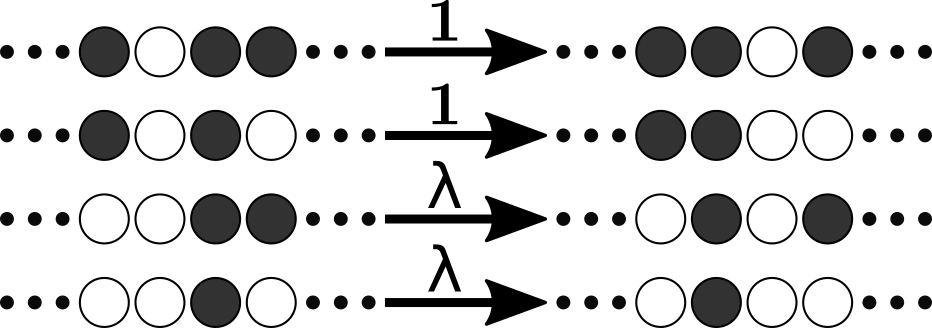
\includegraphics[width=\linewidth]{../tex-src/images/newRates}
    \vspace{-3em}
\end{figure}
The SPM is based upon the symmetric exclusion process~\cite{sugden2007dynamically, Kollmann2003,  Lin2005, Hegde2014, Krapivsky2014, Imamura2017};
it differs from the original in that adjacent particles separate with rate $\lambda$
instead of their normal hopping rate, $1$. It is in fact a version of the KLS model~\cite{Katz1984, Zia2010} in 1-dimension without an applied field, which is itself similar to the dynamics used to analyze the Ising model by
Kawasaki~\cite{PhysRev.145.224}. It seems that this symmetric model has not been researched much (at least in terms of its dynamics) because the model with the applied field is so interesting; however, it seems that the simple symmetric model
exhibits complex unexpected behavior when a concentration gradient is applied. The quantity $\lambda$ parametrizes the ``stickiness'' of the particles; when $\lambda>1$, there is a tendency for particles to repel,
whilst $\lambda < 1$ represents attraction.
It is worth noting that the rates specified in Fig.~\ref{fig:rates} obey detailed balance,  %cite supplimentary materials
with an energy proportional to the number of particle-particle adjacencies
in the system. It seems that space of highly-local exclusion models is so tightly constrained in one-dimension that there is no option but to comply with the detailed balance condition.
%Could stick this in appendix maybe?

%One can show that there exists an isomorphism between this model and the Misanthrope Process~\cite{evansWaclaw2014}. This doesn't help us to solve the model in the kinds of steady flow cases we are mainly interested in due to
%difficulties with the boundary conditions, but it does allow us to show that this model does \textbf{not} exhibit explosive condensation~\cite{waclaw2012explosive}.

